\documentclass[tikz,border=10px]{standalone}
\usepackage{tikz}
\usetikzlibrary{shapes,arrows,positioning,fit,backgrounds}

\begin{document}
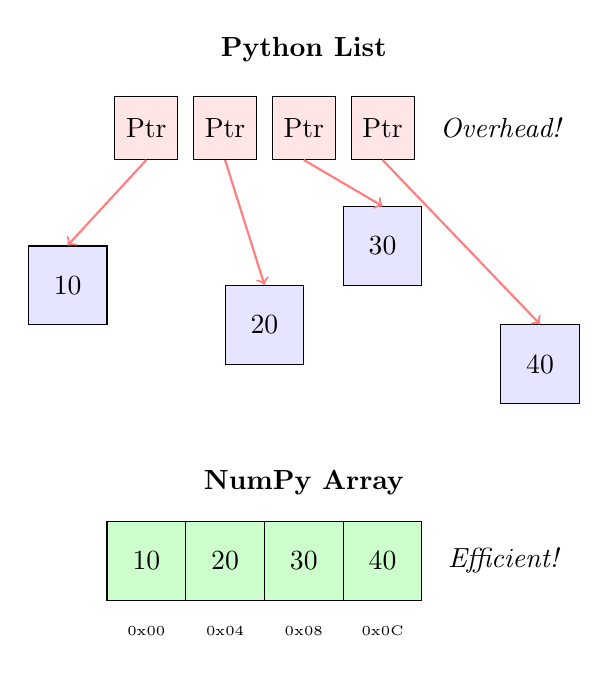
\begin{tikzpicture}[
    node distance=1cm,
    data/.style={draw, rectangle, minimum size=1cm, fill=blue!10},
    pointer/.style={draw, rectangle, minimum size=0.8cm, fill=red!10},
    memory/.style={draw, rectangle, minimum width=1.5cm, minimum height=1cm, fill=gray!10, dashed}
]

    % --- Python List ---
    \node[font=\bfseries] at (2, 4) {Python List};
    
    % List pointers (contiguous block of pointers)
    \node[pointer] (p1) at (0, 3) {Ptr};
    \node[pointer] (p2) at (1, 3) {Ptr};
    \node[pointer] (p3) at (2, 3) {Ptr};
    \node[pointer] (p4) at (3, 3) {Ptr};
    
    \node[right=0.2cm of p4, font=\itshape] {Overhead!};

    % Scattered Objects in Memory
    \node[data] (o1) at (-1, 1) {10};
    \node[data] (o2) at (1.5, 0.5) {20};
    \node[data] (o3) at (3, 1.5) {30};
    \node[data] (o4) at (5, 0) {40};
    
    % Pointers to objects
    \draw[->, thick, red!50] (p1.south) -- (o1.north);
    \draw[->, thick, red!50] (p2.south) -- (o2.north);
    \draw[->, thick, red!50] (p3.south) -- (o3.north);
    \draw[->, thick, red!50] (p4.south) -- (o4.north);

    % --- NumPy Array ---
    \node[font=\bfseries] at (2, -1.5) {NumPy Array};
    
    % Contiguous block of raw data
    \node[data, fill=green!20] (n1) at (0, -2.5) {10};
    \node[data, fill=green!20] (n2) at (1, -2.5) {20};
    \node[data, fill=green!20] (n3) at (2, -2.5) {30};
    \node[data, fill=green!20] (n4) at (3, -2.5) {40};
    
    \node[right=0.2cm of n4, font=\itshape] {Efficient!};
    
    % Label for contiguous block
    \node[below=0.2cm of n1, font=\tiny] {0x00};
    \node[below=0.2cm of n2, font=\tiny] {0x04};
    \node[below=0.2cm of n3, font=\tiny] {0x08};
    \node[below=0.2cm of n4, font=\tiny] {0x0C};

\end{tikzpicture}
\end{document}
